%	This LaTeX file is written by Zhiyang Ong as a template for creating presentation slides.

%	The MIT License (MIT)

%	Copyright (c) <2015> <Zhiyang Ong>

%	Permission is hereby granted, free of charge, to any person obtaining a copy of this software and associated documentation files (the "Software"), to deal in the Software without restriction, including without limitation the rights to use, copy, modify, merge, publish, distribute, sublicense, and/or sell copies of the Software, and to permit persons to whom the Software is furnished to do so, subject to the following conditions:

%	The above copyright notice and this permission notice shall be included in all copies or substantial portions of the Software.

%	THE SOFTWARE IS PROVIDED "AS IS", WITHOUT WARRANTY OF ANY KIND, EXPRESS OR IMPLIED, INCLUDING BUT NOT LIMITED TO THE WARRANTIES OF MERCHANTABILITY, FITNESS FOR A PARTICULAR PURPOSE AND NONINFRINGEMENT. IN NO EVENT SHALL THE AUTHORS OR COPYRIGHT HOLDERS BE LIABLE FOR ANY CLAIM, DAMAGES OR OTHER LIABILITY, WHETHER IN AN ACTION OF CONTRACT, TORT OR OTHERWISE, ARISING FROM, OUT OF OR IN CONNECTION WITH THE SOFTWARE OR THE USE OR OTHER DEALINGS IN THE SOFTWARE.

%	Email address: echo "cukj -wb- 23wU4X5M589 TROJANS cqkH wiuz2y 0f Mw Stanford" | awk '{ sub("23wU4X5M589","F.d_c_b. ") sub("Stanford","d0mA1n"); print $5, $2, $8; for (i=1; i<=1; i++) print "6\b"; print $9, $7, $6 }' | sed y/kqcbuHwM62z/gnotrzadqmC/ | tr 'q' ' ' | tr -d [:cntrl:] | tr -d 'ir' | tr y "\n"



%%%%%%%%%%%%%%%%%%%%%%%%%%%%%%%%%%%%%%%%%%%%%%
%	Preamble

%	Acknowledgement:
%		This is based on a template provided to me by Dott. Francesco Stefanni, from the University of Verona in January 2011.
%
%	Number the slides per section. This makes it easier to track the index of the slides (or number of slides) per section, as opposed to the cumulative number of slides. When I manually track the number of slides for a presentation, each time I refactor the set of slides, I would have to update the slide numbers. I want the computer to do this automatically. Hence, I shall not do this manually.



%	Use the Beamer package to create the presentation slides.
\documentclass[xcolor={usenames,dvipsnames},hyperref={hyperindex,bookmarks}]{beamer}


%%%%%%%%%%%%%%%%%%%%%%%%%%%%%%%%%%%%%%%%%%%%%%
%	Import and Customize LaTeX packages.
\usepackage{beamerthemesplit}


%	Package for typesetting the following symbol: $\mathfrak{S}$
%\usepackage{amssymb}

%\mode<presentation>
%{ \usetheme{boxes} }

%	Select the presentation mode.
\mode<presentation>{
	\usetheme[logos=true,pagenumbers=true,background=true]{Esd}
}
\setbeamercovered{transparent}
%\setbeamercovered{invisible}


%	Import package to facilitate typesetting of algorithms.
\usepackage{listings}

\lstset{
  language=C++,
  tabsize=4,
%  basicstyle=\ttfamily\color{black}\small,
  basicstyle=\ttfamily\color{black},
%  backgroundcolor=\color{lightgray},
%  backgroundcolor=\color{white},
  keywordstyle=\color{Purple}\bfseries,
  identifierstyle=\color{OliveGreen},
  commentstyle=\color{Gray}\itshape,
  stringstyle=\color{CarnationPink},
  showstringspaces=false,
  showtabs=false,
  showspaces=false
}


\definecolor{lightgray}{gray}{0.95}
\font\emailtt=cmtt9

%	Set up configuration for hyperlinks.
%\usepackage[pdftex]{hyperref}	-- Option clash
\hypersetup{
    pdftitle={Making an {\it Arduino} Memory Game},     % title
    pdfauthor={Zhiyang Ong},                 % author
    pdfsubject={IEEE Aggie Mentorship Program}, % subject of the document
    pdfcreator={Creator},                           % creator of the document
    pdfproducer={dvipdft},                          % producer of the document
% Modified by Zhiyang Ong on Feb 7, 2011 to improve the way hyperlinks are colored in these presentation slides
	pdfkeywords={LaTeX, graphics, color},
%    pdfkeywords={C, C++, programming style},        % list of keywords
%
%    bookmarks=true,         % show bookmarks bar?
    unicode=false,          % non-Latin characters in Acrobats bookmarks
    pdftoolbar=true,        % show Acrobats toolbar?
    pdfmenubar=true,        % show Acrobats menu?
    pdffitwindow=false,     % window fit to page when opened
% Modified by Zhiyang Ong on Feb 7, 2011 to improve the way hyperlinks are colored in these presentation slides
	pdfpagemode=UseOutlines,bookmarks, bookmarksopen,
	pdfstartview=FitH, colorlinks, linkcolor=blue, citecolor=blue, urlcolor=red,
%    pdfstartview={Fit},    % fits the width of the page to the window
    pdfnewwindow=true,      % links in new window
% Modified by Zhiyang Ong on Feb 7, 2011 to improve the way hyperlinks are colored in these presentation slides
	colorlinks=red,        % false: boxed links; true: colored links
	linkcolor=red,          % color of internal links
%    colorlinks=false,        % false: boxed links; true: colored links
%    linkcolor=red,          % color of internal links
    citecolor=green,        % color of links to bibliography
    filecolor=magenta,      % color of file links
    urlcolor=red,           % color of external links
    pdfpagemode=FullScreen
    %
    %pdfpagelabels=false
}

%\usepackage[all]{hypcap}




%%%%%%%%%%%%%%%%%%%%%%%%%%%%%%%%%%%%%%%%%%%%%%
%	Added by Zhiyang Ong on Feb 7, 2011 to allow figures to be places side-by-side
%\usepackage{subfigure}









%%%%%%%%%%%%%%%%%%%%%%%%%%%%%%%%%%%%%%%%%%%%%%
%%%%%%%%%%%%%%%%%%%%%%%%%%%%%%%%%%%%%%%%%%%%%%
%%%%%%%%%%%%%%%%%%%%%%%%%%%%%%%%%%%%%%%%%%%%%%
%%%%%%%%%%%%%%%%%%%%%%%%%%%%%%%%%%%%%%%%%%%%%%
%%%%%%%%%%%%%%%%%%%%%%%%%%%%%%%%%%%%%%%%%%%%%%
%%%%%%%%%%%%%%%%%%%%%%%%%%%%%%%%%%%%%%%%%%%%%%
%%%%%%%%%%%%%%%%%%%%%%%%%%%%%%%%%%%%%%%%%%%%%%


%	Quantum Model Checking Is Not Evil: It Is Mandatory For Quantum Robots


%	First slide of the presentation
\title[IEEE Aggie Mentorship Program]
{\huge 
Making an Arduino Memory Game}
\subtitle{A Really Simple Cyber-Physical System}
\author{Zhiyang Ong}
\institute{
	Department of Electrical and Computer Engineering \\
	Dwight Look College of Engineering,\\
	Texas A\&M University \\
	College Station, TX
}
\date{\today}	% (optional)
\subject{Subject Title}

%	This set of presentation slides is based on \cite{Ying2014a}, from my BibTeX research database.







%%%%%%%%%%%%%%%%%%%%%%%%%%%%%%%%%%%%%%%%%%%%%%
%	Do nothing in this section of the LaTeX document

\begin{document}

\begin{frame}
\titlepage
\end{frame}



%	Table of Contents
\AtBeginSection[]		% Do nothing for \subsection*
{
	\begin{frame}
%		\frametitle{\textcolor{yellow}{Table of Contents}}
		\frametitle{Table of Contents}
%		\textcolor{yellow}{\tableofcontents[currentsection]}
		\tableofcontents[currentsection,currentsubsection]
	\end{frame}
}

\AtBeginSubsection[]		% Do nothing for \subsection*
{
\begin{frame}
\tableofcontents[currentsection,currentsubsection]
\end{frame}
}

\section*{Outline}
\begin{frame}
\tableofcontents
\end{frame}



%%%%%%%%%%%%%%%%%%%%%%%%%%%%%%%%%%%%%%%%%%%%%%
%
%	Slides begin HERE!!!
%
%%%%%%%%%%%%%%%%%%%%%%%%%%%%%%%%%%%%%%%%%%%%%%


%%%%%%%%%%%%%%%%%%%%%%%%%%%%%%%%%%%%%%%%%%%%%%
%	Preamble

%	Slide #1
\section{Preamble}
\begin{frame}
	\frametitle{Acknowledgments}
	Dott. Francesco Stefanni, University of Verona \\
	\ \\
	IEEE TAMU Officers
	\begin{itemize}
	\item Maria Theresia Tyas
	\item Millie Kriel
	\item Polina Golikova
	\end{itemize}
	\ \\
	\ \\
	Reference: Jerepondumie, ``Make an Arduino Memory Game,'' in {\it Hackster.io}, Hackster, Inc., San Francisco, CA, September 15, 2017. Available online from {\it Hackster.io} at: \url{https://www.hackster.io/Jerepondumie/make-an-arduino-memory-game-73f55e}; February 18, 2018 was the last accessed date.
\end{frame}



%	Slide #2
\frame
{
	\frametitle{Warnings!!!}

	``The code is rather buggy; use is at own risk.'' \\
	-- Donald Chai \\
	\ \\
	``Beware of bugs in the above code. \\
	I have only proved it correct, not tried it.'' \\
	-- Donald E. Knuth \ \\
	\ \\
	Unlike the Fantastic and Fabulous Ms. Millie Kriel, I have yet to try out this tutorial.
}




%	Slide #3
\frame
{
	\frametitle{Ice Breaker}

	Name \\
	\ \\
	%What are some of your favorite study techniques? \\
	What suggestions do you have for freshmen who are deciding what they can do this summer? \\
	\ \\
	What are some of your favorite study techniques for circuit analysis (ECEN 214) and logic design (ECEN 248)? \\
}







%%%%%%%%%%%%%%%%%%%%%%%%%%%%%%%%%%%%%%%%%%%%%%
%	Summary
\section{Summary}

%	Slide 1
\frame
{
	\frametitle{Summary}

	\begin{itemize}
	\item Cyber-physical system design
	\item Implement a memory game on the {\it Arduino} platform: %\vspace{-0.3cm}
		\begin{itemize} %\itemsep -2pt
		\item Implement simple analog circuit design on a breadboard
		\item Connect breadboard to the {\it Arduino} platform
		\item Program the microcontroller on the {\it Arduino} platform
		\end{itemize}
	\item Play the memory game
	\item Repeat previous steps ad infinitum until you get bored.
	\end{itemize}
}






%%%%%%%%%%%%%%%%%%%%%%%%%%%%%%%%%%%%%%%%%%%%%%
%	Required Components and Software Applications/Services
\section{Required Components and Software Applications/Services}


%	Slide 1
\frame
{
	\frametitle{Required Components and Software Applications/Services}

	\begin{itemize}
	\item Software applications/services:
		\begin{itemize}
		\item {\it Arduino} IDE
		\end{itemize}
	\end{itemize}

	\begin{table}[htdp]
\caption{Hardware components}
\label{tab:Table}
	\begin{center}
		\begin{tabular}{|c|c|c|c|}
		\hline
		{\it Arduino} UNO {\rm \&}\ {\it Genuino} UNO & 1 \\
		\hline
		{\it SparkFun} 330 ohm resistors & 4 \\
		\hline
		{\it SparkFun} 10k ohm resistors & 4 \\
		\hline
		{\it SparkFun} Assorted LEDs & 4 \\
		(4 LEDs of different colors) & \\
		\hline
		{\it SparkFun} Mini speaker & 1 \\
		(Recommended, not required) & \\
		\hline
		{\it SparkFun} breadboard (Full size) & 1 \\
		\hline
		Jumper wires (generic) & 1 \\
		\hline
		\end{tabular}
	\end{center}
\end{table}

}


%%%%%%%%%%%%%%%%%%%%%%%%%%%%%%%%%%%%%%%%%%%%%%
%	Schematic for Hardware Implementation
\section{Schematic for Hardware Implementation}

%	Slide 1
\frame
{
	\frametitle{Schematic for Hardware Implementation}

\begin{figure}[h]
\centering 
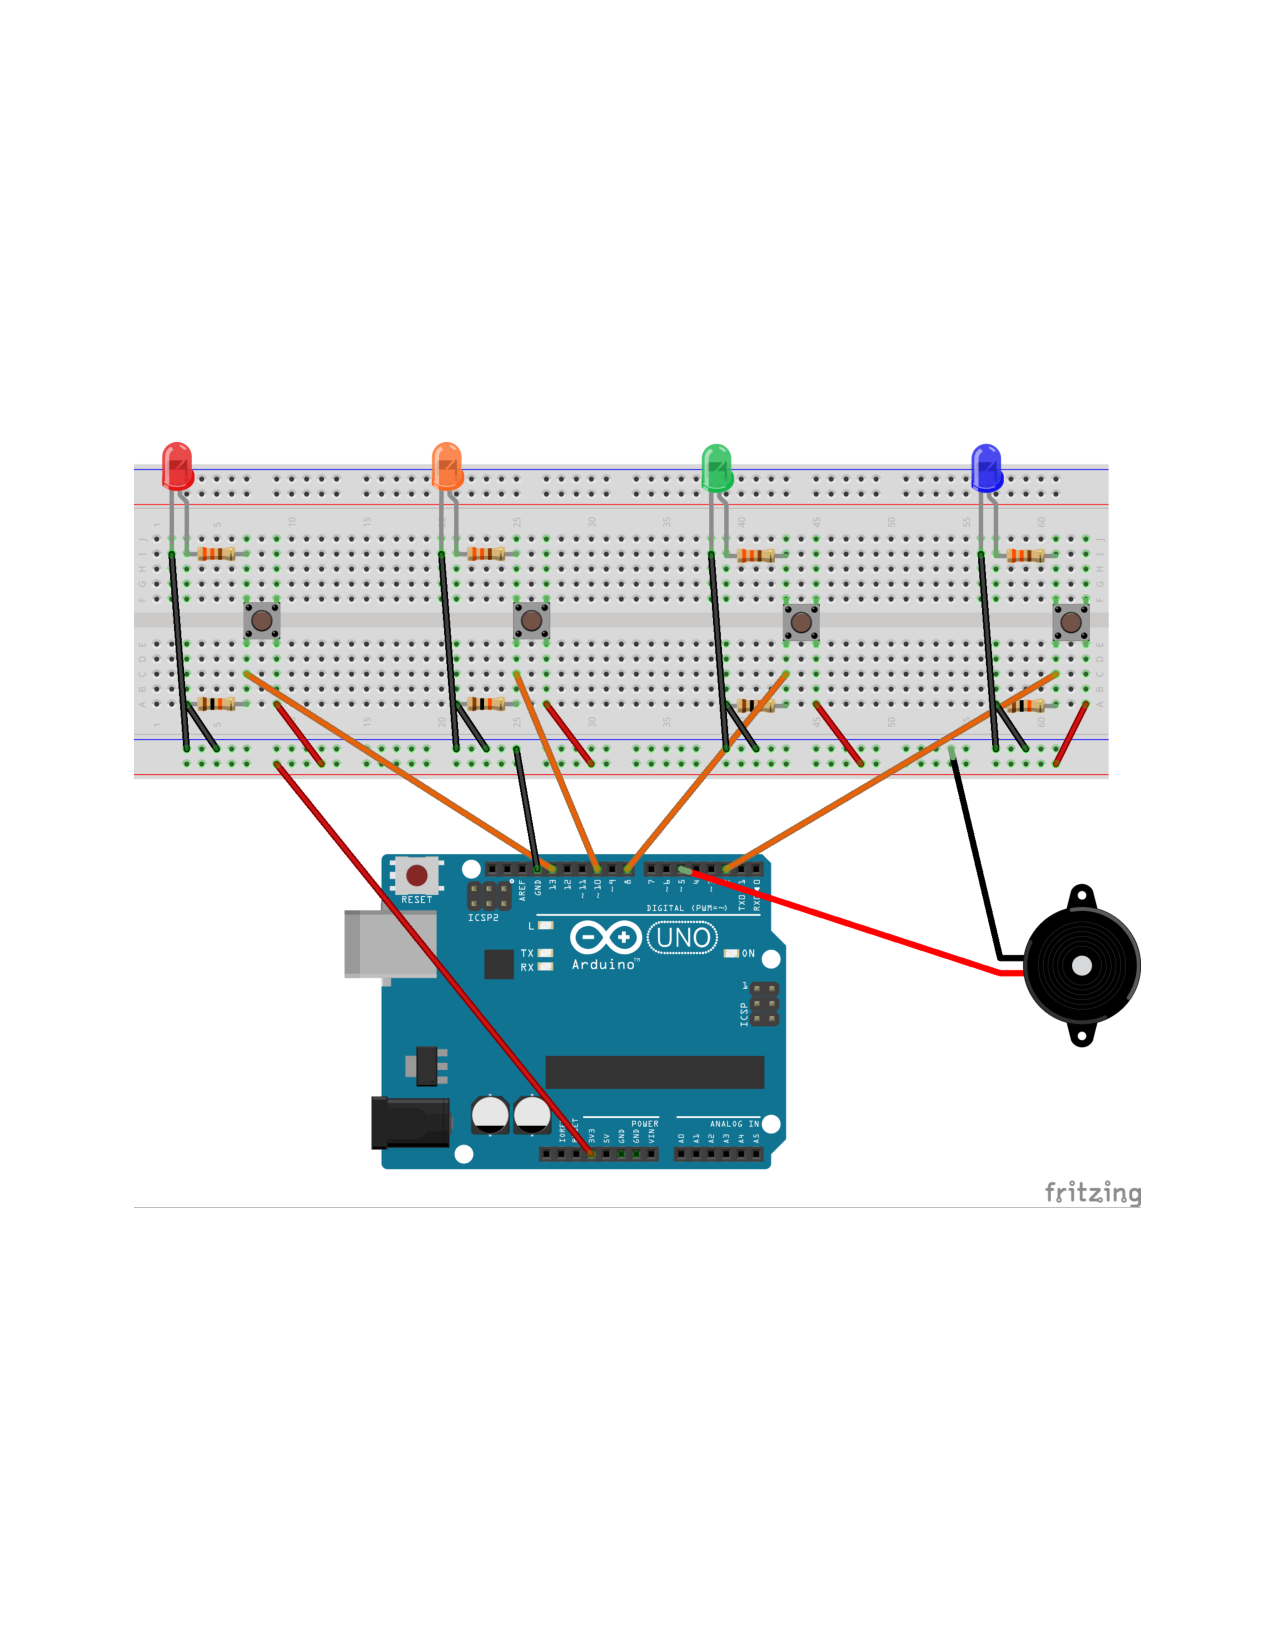
\includegraphics[height=2.2in]{./pics/hw-implementation-simple-simon}
\caption{Schematic for Hardware Implementation on the Breadboard}
\label{fig:hwimplementationsimplesimon}
\end{figure}
}


%%%%%%%%%%%%%%%%%%%%%%%%%%%%%%%%%%%%%%%%%%%%%%
%	Source Code for Software Implementation
\section{Source Code for Software Implementation}

%	Slide 1
\frame
{
	\frametitle{Source Code for Software Implementation}

\begin{figure}[h]
\centering 
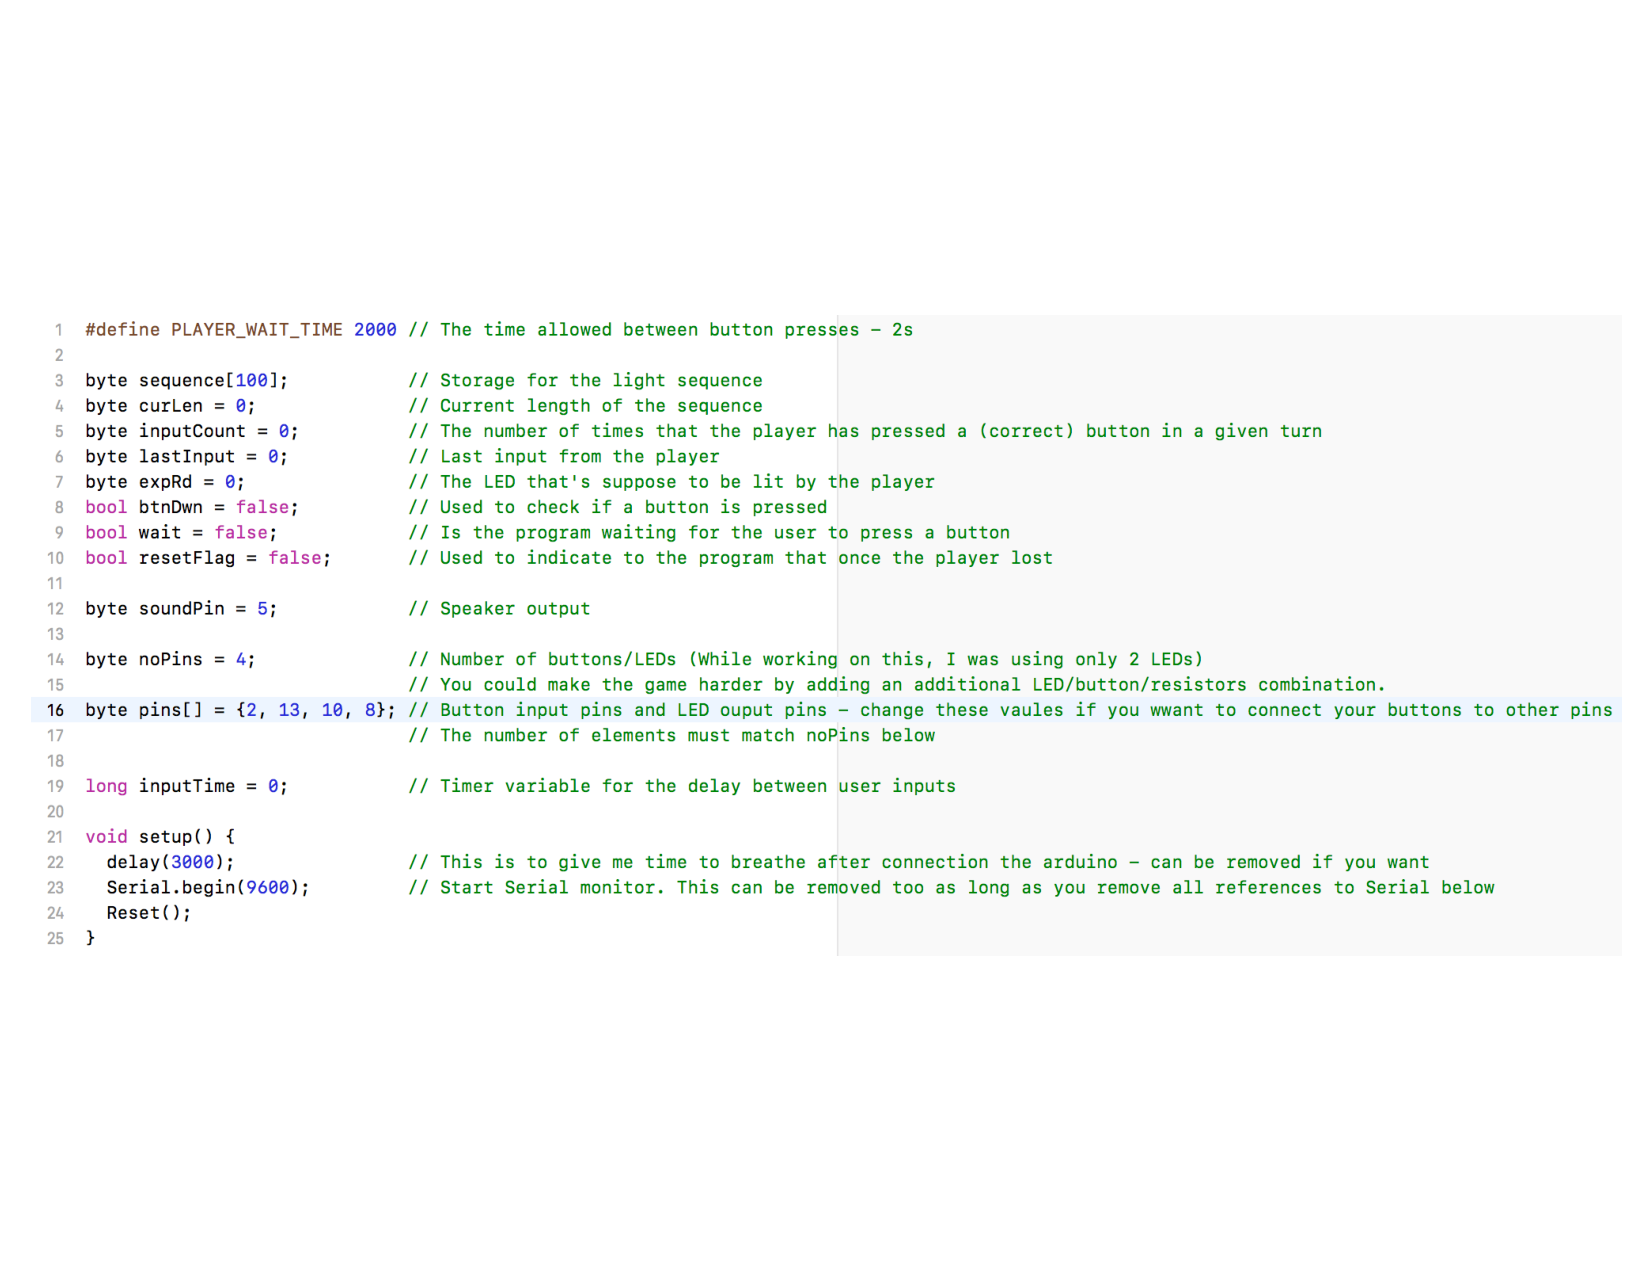
\includegraphics[height=1.80in]{./pics/sw-setup}
\caption{Software to Set Up the Memory Game}
\label{fig:swsetup}
\end{figure}
}



%	Slide 2
\frame
{
	\frametitle{Source Code for Software Implementation (2)}

\begin{figure}[h]
\centering 
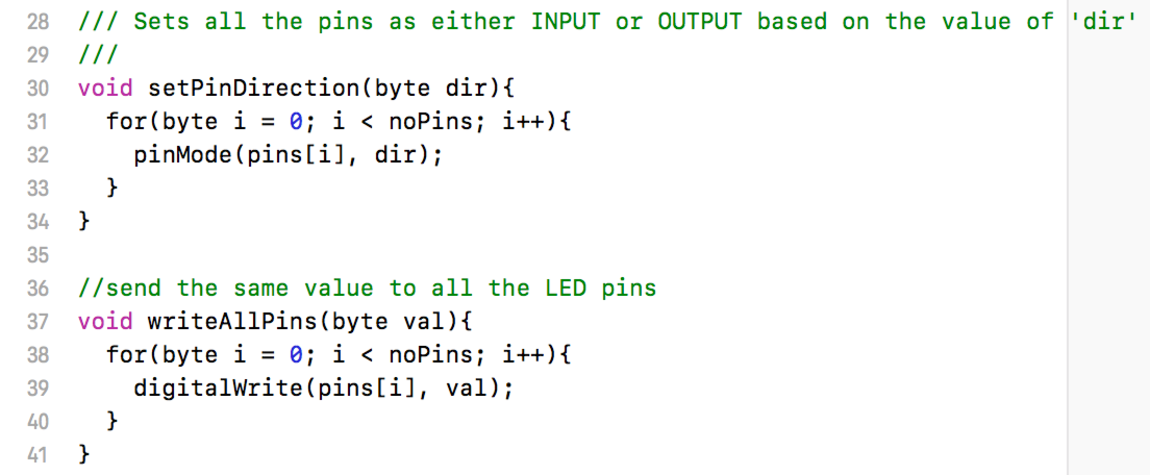
\includegraphics[height=1.90in]{./pics/sw-infrastructure}
\caption{Software Infrastructure for the Memory Game (2)}
\label{fig:swinfrastructure}
\end{figure}
}




%	Slide 3
\frame
{
	\frametitle{Source Code for Software Implementation (3)}

\begin{figure}[h]
\centering 
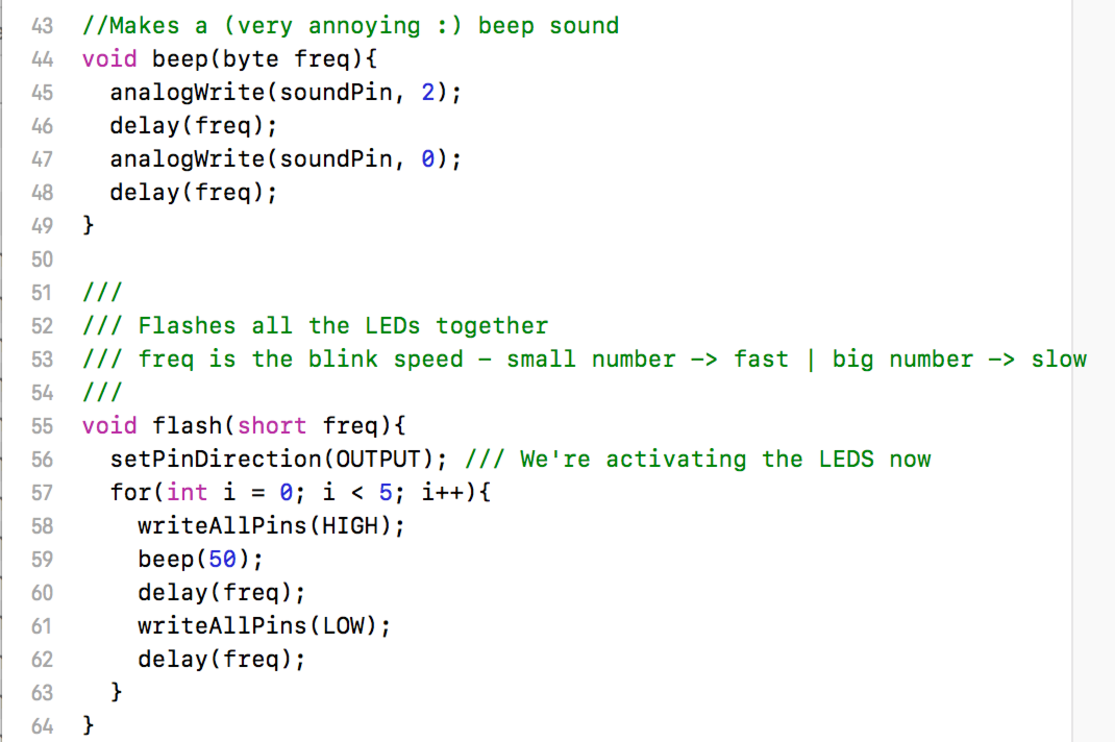
\includegraphics[height=2.2in]{./pics/sw-infrastructure2}
\caption{Software Infrastructure for the Memory Game (3)}
\label{fig:swinfrastructure2}
\end{figure}
}







%	Slide 3
\frame
{
	\frametitle{Source Code for Software Implementation (4)}

\begin{figure}[h]
\centering 
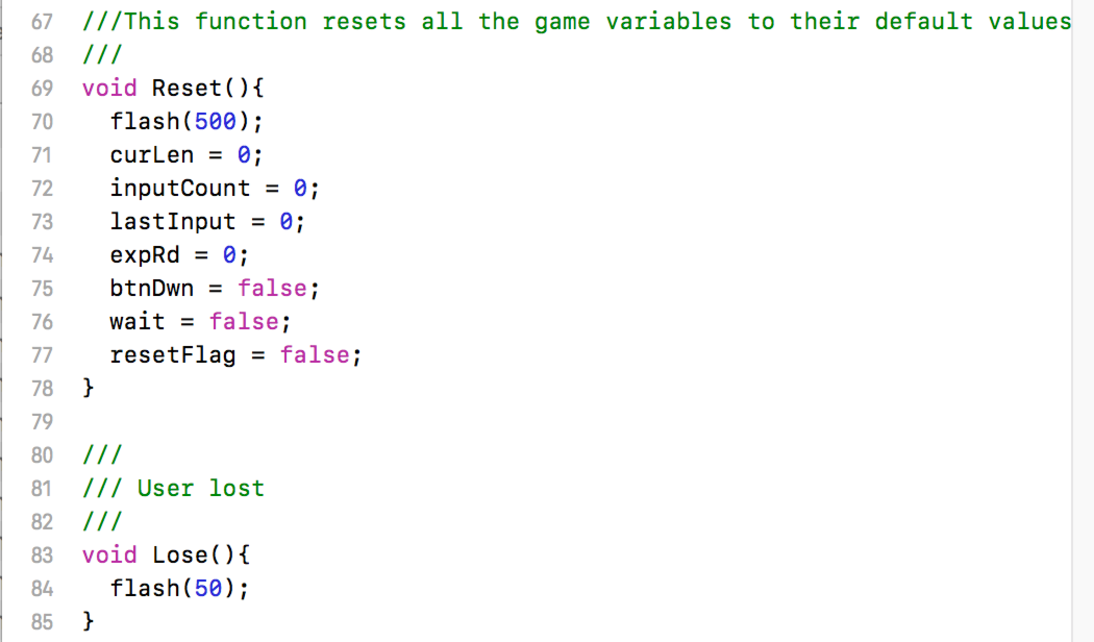
\includegraphics[height=2.2in]{./pics/sw-infrastructure3}
\caption{Software Infrastructure for the Memory Game (4)}
\label{fig:swinfrastructure3}
\end{figure}
}



\frame
{
	\frametitle{Source Code for Software Implementation (5)}

\begin{figure}[h]
\centering 
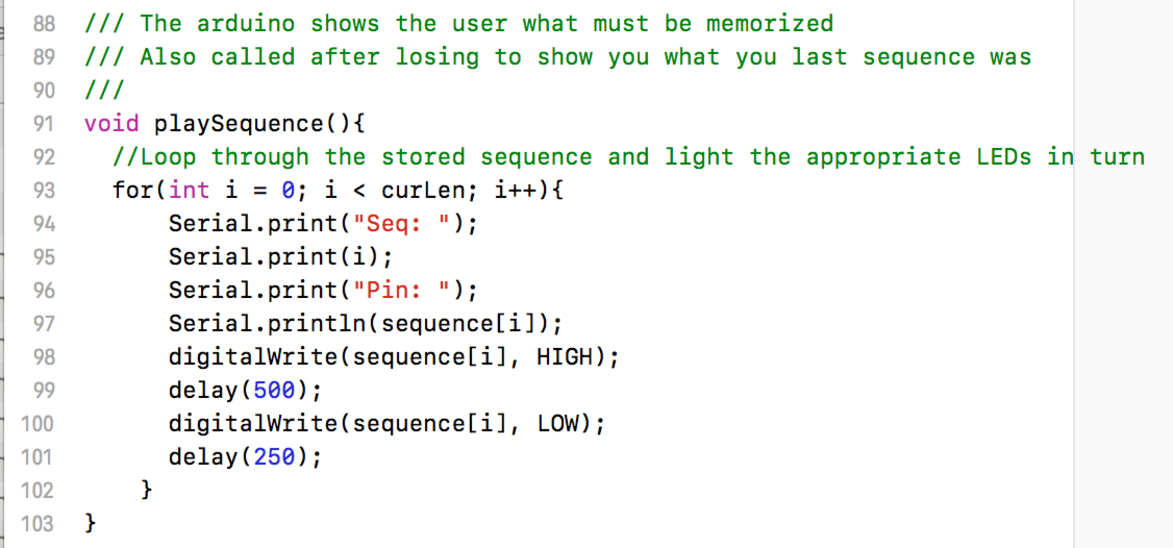
\includegraphics[height=2.0in]{./pics/sw-infrastructure4}
\caption{Software Infrastructure for the Memory Game (5)}
\label{fig:swinfrastructure4}
\end{figure}
}

\frame
{
	\frametitle{Source Code for Software Implementation (6)}

\begin{figure}[h]
\centering 
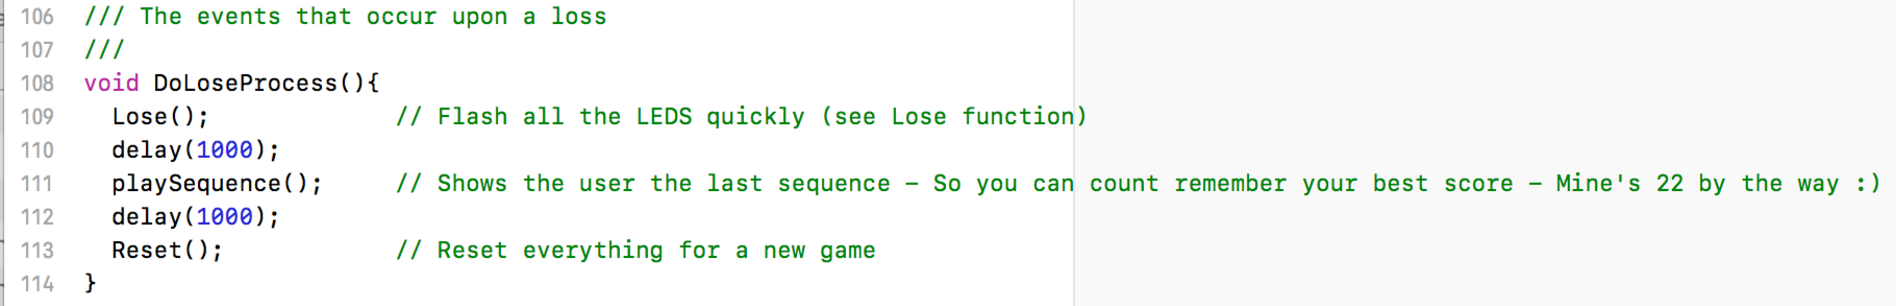
\includegraphics[height=0.7 in]{./pics/sw-infrastructure5}
\caption{Software Infrastructure for the Memory Game (6)}
\label{fig:swinfrastructure5}
\end{figure}
}











%%%%%%%%%%%%%%%%%%%%%%%%%%%%%%%%%%%%%%%%%%%%%%
%	Additional Comments
\section{Additional Comments}

%	Slide 4
\frame
{
	\frametitle{Additional Comments}

	\begin{itemize}
	\item Almost all previous work use model checking to verify quantum communication protocols
	\item Use quantum process algebra to verify quantum communication systems, including quantum error correction codes
	\item Use simulation tools for quantum systems to verify their behavior/functionality, especially their correctness and safety properties
	\item Quantum partially observable Markov decision processes (QOMDPs), which are introduced by (Barry, Barry, and Aaronson, 2014), only care about the reachability of a single state (i.e., goal state).: %\vspace{-0.2cm}
		\begin{itemize} \itemsep -2pt
		\item The paper does not specifically address the reachability of invariant subspaces.
		\item Goal-state reachability is undecidable for QOMDPs.
		\end{itemize}
	\end{itemize}
}

















%%%%%%%%%%%%%%%%%%%%%%%%%%%%%%%%%%%%%%%%%%%%%%
%\section{References}
%
%\frame
%{
%	\frametitle{References}
%
%%	\begin{itemize}
%%	\item \cite{Weng2011}
%%	\end{itemize}
%%}
%
%
%	{\linespread{1}
%	%\bibliographystyle{IEEEtran}
%	\bibliographystyle{plain}
%	%\bibliography{./others/references}
%	%\bibliography{/data/others/notes/references}
%	\bibliography{/data/research/antipastobibtex/references}
%	%\addcontentsline{toc}{chapter}{Bibliography}
%	}
%}

\end{document}


%
%	Trying to delay the not-uncommon path of engineering Ph.D.s who end up becoming "PowerPoint engineers"... Hopefully, slapping together a bunch of presentation slides to talk about any topic in any reasonable finite amount of time is not the most useful skill that I would learn as a grad student... Hey, at least I did it in LaTeX/Beamer!!!






 